\chapter{The EM-algorithm}

\newcommand{\timedomain}{[0, \infty)}

\section{Introduction}

We motivate and present the EM (expectation-maximization) algorithm, an algorithm used for approximately computing parameter values for probability distributions in maximum-likelihood estimation. The reader is expected to have knowledge of undergraduate probability theory and to be familiar with maximum-likelihood estimation.

The presentation is divided in three parts. Section~\ref{sec:vegan_flea} presents an optimization problem regarding a vegan flea. We present an algorithm that finds an approximate solution and provides intuitions to understand why the EM-algorithm works. Section~\ref{sec:movie_recommendation} presents the problem of building a simple movie recommendation system. We show that movie ratings can be understood as samples from a probabilistic model that is defined by a set of multivariate Bernoulli distributions. Estimating the parameters of these distributions via maximum-likelihood turns out to be very hard using analytical methods. In Section~\ref{sec:em_algo}, we show that this maximum-likelihood estimation problem is an instance of the vegan-flea optimization problem and derive the EM-algorithm from the approximation algorithm presented in Section~\ref{sec:vegan_flea}.

\section{The vegan-flea optimization problem}
\label{sec:vegan_flea}

\subsection{The dog}

We introduce a two-dimensional dog, depicted in Figure~\ref{fig:dog}. Although, in practice, dogs are three-dimensional entities, a two-dimensional dog makes easier the presentation of some ideas later. Observe that this two-dimensional dog has only two legs, since two legs suffice to keep balance, and one eye, since there is no need for perspectives in a two-dimensional space. 

Figure~\ref{fig:dog_close_up} shows some of the dog's cardiovascular system. Observe that a blood vessel of a two-dimensional being does not have the shape of a cilinder. They still naturally expand when a surge of blood flows from a heart's pump. For the rest of these notes we focus only on a small area of this figure; namely, the tiny green square shown in the figure.

\begin{figure}
\centering
\begin{subfigure}[b]{0.45\textwidth}
\centering
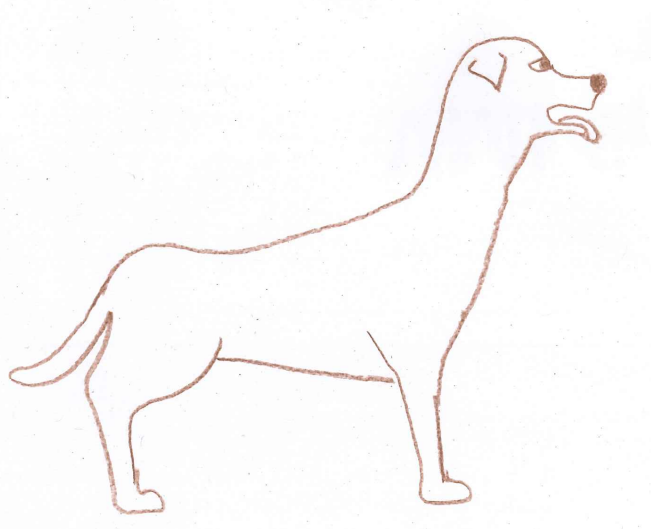
\includegraphics[width=\textwidth]{\dir/dog}
\caption{A two-dimensional dog.}
\label{fig:dog}
\end{subfigure}

\begin{subfigure}[p]{0.45\textwidth}
\centering
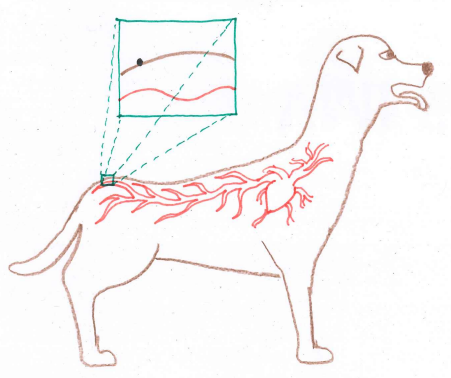
\includegraphics[width=\textwidth]{\dir/dog_close_up}
\caption{A part of the dog's (two-dimensional) cardiovascular system.}
\label{fig:dog_close_up}
\end{subfigure}

\begin{subfigure}[p]{0.45\textwidth}
\centering
        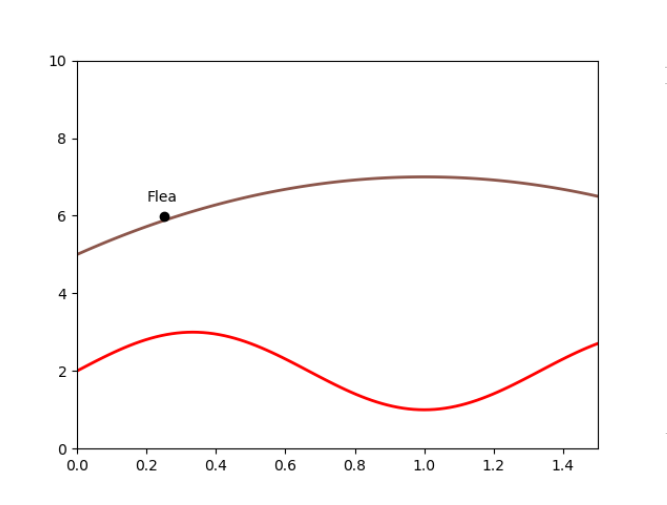
\includegraphics[width=\textwidth]{\dir/vegan_mosquito_start}
        \caption{The flea, the skin, and the upper border of a blood vessel.}
        \label{fig:skin_vessel_simp}
\end{subfigure}
\caption{}
\label{fig:dog_vessel_flea}
\end{figure}

Figure~\ref{fig:skin_vessel_simp} shows the area marked by the green square in detail. We have placed some Cartesian axes there for reference. There is a flea at coordinates (0.25, 6). The dog's skin is the brown curve, and the upper border of a blood vessel is the red curve. Observe that, in a two-dimensional space, skins are lines instead of surfaces.

\subsection{The skin and the blood vessel's upper border}

\newcommand{\skin}{\mathit{skin}}
\newcommand{\vessel}{\mathit{vessel}}

We now mathematically model the skin and the blood vessel's upper border.
Let $\skin : [0, 1] \times \timedomain \to \mathbb{R}$, and $\vessel : [0, 1] \times \timedomain \to \mathbb{R}$ be two functions. For $t \in \timedomain$, let $\skin(\cdot, t) : [0, 1] \to \mathbb{R}$ be the function that maps $x$ to $\skin(x, t)$. We define the function $\vessel(\cdot, t)$ analogously. Intuitively, for $t \in \timedomain$, the functions $\skin(\cdot, t)$ and $\vessel(\cdot, t)$ describe the skin and the blood vessel's upper border at time $t$, as depicted in Figure~\ref{fig:skin_vessel}. Hence, $\skin(x, t) \geq \vessel(x, t)$, for any $(x, t) \in [0, 1] \times \timedomain$. 
%Although the skin surface and the blood vessel should be modeled in $\mathbb{R}^3$, we restrict ourselves to $\mathbb{R}^2$ to keep the presentation simple. 
Observe that $\skin(\cdot, t)$ and $\vessel(\cdot, t)$ vary with $t$. This is to model the fact that blood flows through the vessel and, consequently, makes the skin surface and the blood vessel's upper border vary with time. The animated .gif file attached with these notes\footnote{\url{https://people.inf.ethz.ch/ccarlos/assets/em/vegan\_flea.gif}} illustrate the setting. We strongly encourage the reader to look the .gif file before proceeding.

\begin{figure}
    \centering
    \begin{subfigure}[b]{0.8\textwidth}
        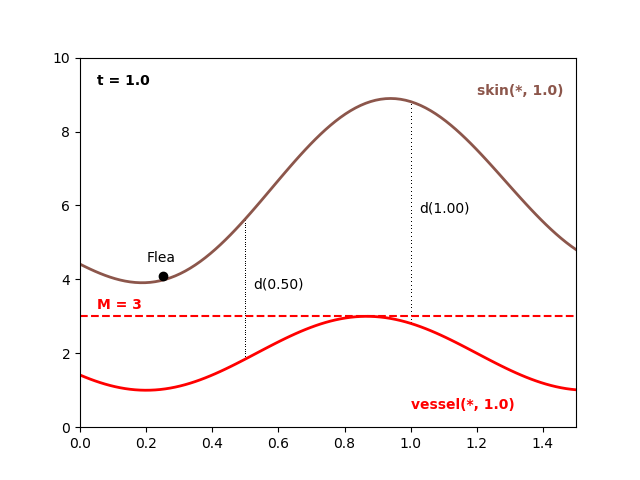
\includegraphics[width=\textwidth]{\dir/vegan_mosquito_40}
        \caption{Skin and blood vessel at $t = 1$}
        \label{fig:skin_vessel_t0}
    \end{subfigure}
    ~ %add desired spacing between images, e. g. ~, \quad, \qquad, \hfill etc. 
      %(or a blank line to force the subfigure onto a new line)
      
    \begin{subfigure}[b]{0.8\textwidth}
        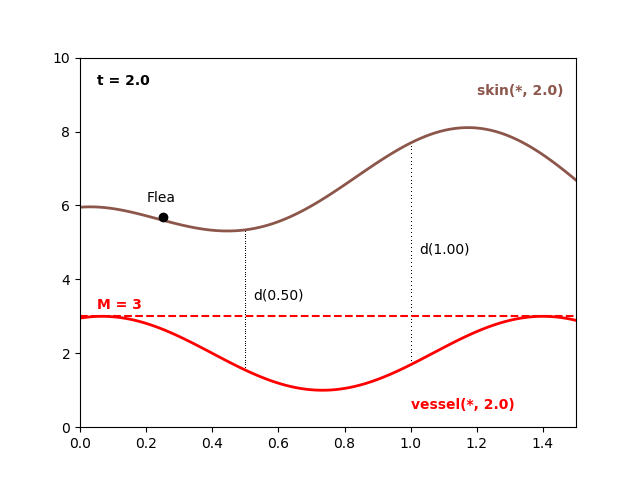
\includegraphics[width=\textwidth]{\dir/vegan_mosquito_80}
        \caption{Skin and blood vessel at $t = 2$}
        \label{fig:skin_vessel_t1}
    \end{subfigure}
    ~ %add desired spacing between images, e. g. ~, \quad, \qquad, \hfill etc. 
    %(or a blank line to force the subfigure onto a new line)
    \caption{An illustration of the functions $\skin(\cdot, t)$ and $\vessel(\cdot, t)$, for $t \in \{1, 2\}$.}\label{fig:skin_vessel}
\end{figure}

\begin{assumption}
We assume that for any $x \in [0, 1]$ and any two time points $t_1, t_2 \in \timedomain$, $\skin(x, t_1) - \vessel(x, t_1) = \skin(x, t_2) - \vessel(x, t_2)$. 
\label{asm:unelastic_skin}
\end{assumption}

This assumption states that the skin surface changes by the same amount that the blood vessel's upper border changes. This allows us to define a function $d$ such that $d(x) = \skin(x, t) - \vessel(x, t)$, for any $x \in [0, 1]$ and $t \in \timedomain$.

Blood flows periodically through the vessel and therefore makes the vessel shape change. Moreover, we assume the following:

\begin{assumption}
For any $x \in [0,1]$ and any $t \in \timedomain$, there is $t' \geq t$ such that $\vessel(x, t') = \max_{x'}\vessel(x', t')$.
\label{asm:periodic_flow}
\end{assumption}

If you observe the .gif animation, you can see that we defined a constant $M$. You can also see that, for any $x$ and any $t$, $\vessel(x, t) \leq M$ and that there is $t' \geq t$ such that $\vessel(x, t') = M$. We could then make Assumption~\ref{asm:periodic_flow} stronger by stating that, for any $x \in [0, 1]$ and any $t \in \timedomain$, $\vessel(\cdot, t)$ is bounded by $M$ and that there is $t' \geq t$ such that $\vessel(x, t) = M$. However, Assumption~\ref{asm:periodic_flow} is enough for our purposes. Moreover, it is weaker and, hence, more general.

\subsection{The vegan flea}

Imagine now that there is a flea resting on the skin surface at $(x_0, \skin(x_0, 0))$, for some $x_0 \in [0, 1]$. The flea has decided to become vegan and wishes to be as far away from the blood vessel as possible, to avoid the temptation of the blood. More precisely, the flea's goal is the following.

\begin{objective}
Compute a value $x^*$ that maximizes $d$.
\end{objective}

A look at the .gif file shows that $x^* = 1.0$. This is easy for us as we, three-dimensional creatures, have an omniscient view of the flea's universe. The flea, however, cannot see that as she knows nothing about $\vessel$. In spite of this, we illustrate how the flea can partially achieve its objective.

We make two assumptions about the flea's computation abilities.

\begin{assumption}
For any $t \in \timedomain$, the flea can efficiently compute 
%
$$x^* = \arg\max_{x'}\skin(x, t).$$
%
\label{asm:flea_m_step}
\end{assumption}

This assumption bases on the idea that the flea can see the dog's skin and can therefore maximize $\skin(\cdot, t)$. The next assumption states that the flea, located at $(x_0, (\skin(x_0, 0)))$, can identify the moment $t'$ when $\vessel(x_0, t') = M$, the maximum of $\vessel(\cdot, t)$. 

\begin{assumption}
For any $x \in [0, 1]$ and any $t \in \timedomain$, the flea can efficiently compute some $\hat{t} \geq t$ such that $\vessel(x, \hat{t}) = \max_{x'}\vessel(x', \hat{t})$.
\label{asm:flea_e_step}
\end{assumption}
%
We give some justification for this assumption. Blood flows through the vessel in a periodic way and $\skin(\cdot, t)$ changes in the same way as $\vessel(\cdot, t)$ does. Hence, the flea can learn the blood pulse and then wait for a time $\hat{t}$ where $\vessel(x_0, \hat{t}) = M$.

\subsection{An approximate maximization algorithm}
\label{sub:approx_max_algo}

We describe a strategy by which the flea can compute a value $x^*$ such that $d(x^*) \geq d(x_0)$, where $(x_0, \skin(x_0, 0))$ is the flea's current position.
%
\begin{description}
\item[[E-step]] The flea waits for a time $\hat{t}$ at which $\vessel(x_0, \hat{t}) = \max_x\vessel(x, \hat{t})$ (Figure~\ref{fig:vegan_flea_opti_s1}). This is possible by Assumption~\ref{asm:flea_e_step}.
\item[[M-step]] At time $\hat{t}$, the flea computes a value $x^*$ such that 
%
$$x^* = \arg\max_{x} \skin(x, \hat{t}).$$
%
(Figure~\ref{fig:vegan_flea_opti_s2}). This is possible by Assumption~\ref{asm:flea_m_step}.
\item[[Move]] The flea moves to $(x^*, \skin(x^*, \hat{t}))$ (Figure~\ref{fig:vegan_flea_opti_s3}). 
\end{description}
%
Figure~\ref{fig:vegan_flea_proof_non_decrease} illustrates why $d(x^*) \geq d(x_0)$. Observe that $\skin(x^*, \hat{t}) \geq \skin(x_0, \hat{t})$, since $x^*$ is a maximum of $\skin(\cdot, \hat{t})$. Observe also that $\vessel(x^*, \hat{t}) \leq \vessel(x_0, \hat{t})$, since $\vessel(x_0, \hat{t})$ is a maximum of $\vessel(\cdot, \hat{t})$. Hence, $d(x^*) = \skin(x^*, \hat{t}) - \vessel(x^*, \hat{t}) \geq \skin(x_0, \hat{t}) - \vessel(x_0, \hat{t}) = d(x_0)$.

\begin{figure}
\centering
\begin{subfigure}[b]{0.6\textwidth}
\centering
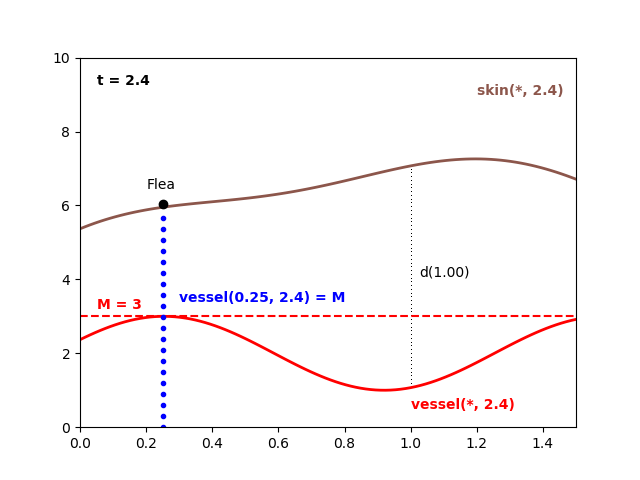
\includegraphics[width=\textwidth]{\dir/vegan_mosquito_e_step}
\caption{Step 1.}
\label{fig:vegan_flea_opti_s1}
\end{subfigure}

\begin{subfigure}[p]{0.6\textwidth}
\centering
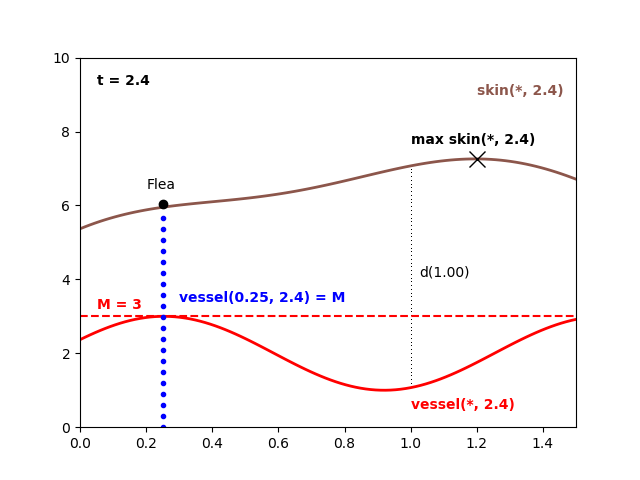
\includegraphics[width=\textwidth]{\dir/vegan_mosquito_m_step_before_jump}
\caption{Step 2.}
\label{fig:vegan_flea_opti_s2}
\end{subfigure}

\begin{subfigure}[p]{0.6\textwidth}
\centering
        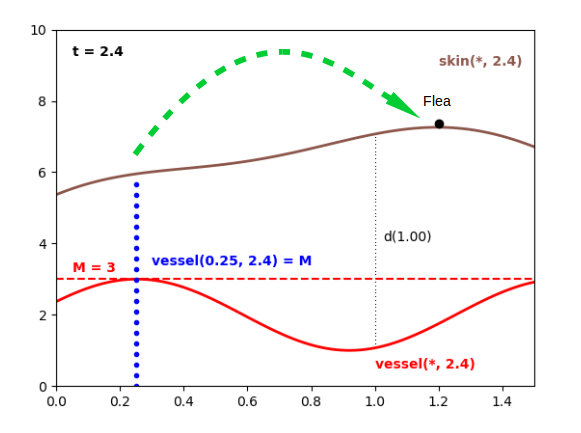
\includegraphics[width=\textwidth]{\dir/vegan_mosquito_m_step_after_jump}
        \caption{Step 3.}
        \label{fig:vegan_flea_opti_s3}
\end{subfigure}
\caption{}
\label{fig:vegan_flea_opti_algo}
\end{figure}

\begin{figure}
\centering
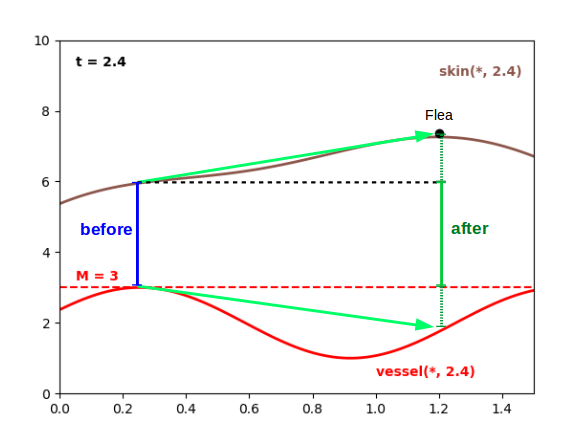
\includegraphics[width=0.6\textwidth]{\dir/vegan_mosquito_proof_nondecrease}
\caption{}
\label{fig:vegan_flea_proof_non_decrease}
\end{figure}

Notice that the flea can set $x_0 = x^*$ and repeat this procedure to find another value $x^{**}$ such that $d(x^{**}) \geq d(x^*)$. The flea can repeat this process as long as the computed values increase $d$. 

We summarize these insights into Algorithm~\ref{algo:vegan_flea}, which computes a sequence of values $x_0$, $x_1, \ldots$ such that $d(x_0) \leq$ $d(x_1) \leq \ldots$ Observe that this algorithm converges. 

One can also relax the assumptions above so that the algorithm works even when $\vessel$ and $\skin$'s domains are a product $\mathcal{X} \times \mathcal{T}$ of any two sets $\mathcal{X}$ and $\mathcal{T}$.

\begin{algorithm}[h!]
\caption{}
\label{algo:vegan_flea}
\begin{algorithmic}[1]
\Require{$\mathcal{X}$ and $\mathcal{T}$ two sets and real functions $d$, $\vessel$, and $\skin$ satisfying the following.
\begin{description}
\item[A1]\label{asm:gen_dist_indep_time} $d(x) = \skin(x, t) - \vessel(x, t)$, for any $x \in \mathcal{X}$ and $t \in \mathcal{T}$.
\item[A2]\label{asm:gen_e_asm} For any $x \in \mathcal{X}$, one can efficiently compute $\hat{t} \in \mathcal{T}$ such that $\vessel(x, \hat{t}) = \max_{x'}\vessel(x', \hat{t})$.
\item[A3]\label{asm:gen_m_asm} For any $t \in \mathcal{T}$, one can efficiently compute $\arg\max_x \skin(x, t)$. 
\end{description}}
\Function{DistanceMax}{$\vessel : \mathcal{X} \times \mathcal{T} \to \mathbb{R}$, $\skin : \mathcal{X} \times \mathcal{T} \to \mathbb{R}$}
	\State {Choose any $x_0 \in \mathcal{X}$.}
	\For {$i = 0, 1, \ldots$}
		\State {\textbf{[E-step]} Compute $\hat{t} \in \mathcal{T}$ s.t. $\vessel(x_0, \hat{t}) = \max_x\vessel(x, \hat{t})$.}
		\State {\textbf{[M-step]} Compute $x^* = \arg\max_x \skin(x, \hat{t})$.}
		\State Print $x^*$ and $d(x^*)$.
		\State $x_0 \gets x^*$.
	\EndFor
\EndFunction
\end{algorithmic}
\end{algorithm}
%

With an argumentation similar to the one above, one can prove that $d(x^*)$ never decreases between two iterations of Algorithm~\ref{algo:vegan_flea}'s loop.

\section{Building a movie-recommendation system with a mixture of multivariate Bernoulli distributions}
\label{sec:movie_recommendation}

\begin{table}[hbtp]
  \begin{tabulary}{\textwidth}{|r|C|C|c|C|C|C|}
\hline
& Star Wars & Star Trek & Titanic & Pretty Woman & 007 & Mission Impossible\\
\hline
\hline
Alice & $\checkmark$ & $\checkmark$ & $\times$ & $\times$ & $\times$ & $\times$ \\
\hline
Bob & $\checkmark$ & $\checkmark$ & $\times$ & $\times$ & $\times$ & $\times$ \\
\hline
Carlos & $\times$ & $\times$ & $\checkmark$ & $\checkmark$ & $\times$ & $\times$\\
\hline
David & $\times$ & $\times$ & $\checkmark$ & $\checkmark$ & $\times$ & $\times$\\
\hline
Ellen & $\times$ & $\times$ & $\checkmark$ & $\times$ & $\times$ & $\checkmark$\\
\hline
Fabian & $\times$ & $\times$ & $\checkmark$ & $\checkmark$ & $\times$ & $\times$\\
\hline
Gabriel & $\checkmark$ & $\checkmark$ & $\times$ & $\times$ & $\checkmark$ & $\checkmark$ \\
\hline
Hector & $\checkmark$ & $\times$ & $\times$ & $\times$ & $\checkmark$ & $\checkmark$ \\
\hline
Ian & $\checkmark$ & $\checkmark$ & $\times$ & $\times$ & $\checkmark$ & $\checkmark$ \\
\hline
Zelya & $\checkmark$ & $\times$ & $\checkmark$ & $\times$ & $\times$ & $\checkmark$ \\
\hline
John & ? & ? & ? & $\checkmark$ & ? & ? \\
\hline

  \end{tabulary}  
    \caption{Ratings from 10 individuals for 6 movies. According to the table, everyone who likes Pretty Woman also liked Titanic. Therefore, it is likely that John would also like Titanic.}
\label{tab:movie_ratings}
\end{table}
%

Table~\ref{tab:movie_ratings} shows the ratings that 10 (fictitious) individuals gave to 6 popular movies. To keep it simple, we assume only binary ratings (good or bad). After a close look to the ratings, the reader can see that Alice and Bob have the exact same taste for movies: \emph{sci-fi} movies. The next four people have a strong interest for \emph{romantic} movies. The next three people like sci-fi and action movies. Zelya's tastes seem to be different from everyone else.

Consider now John, he likes Pretty Woman, but does not like Star trek. He has not seen any of the other movies. What movie could we recommend to him? Since he likes Pretty Woman and everyone who liked Pretty Woman also liked Titanic, we can recommend him to watch Titanic.

From all $2^6$ combinations of ratings, the table contains only a few of them. Moreover, a large majority of the people in the table seem to belong to one of very few taste categories: sci-fi, romantic, or sci-fi+action. Real life is not so different: a large majority of people can partitioned into very few categories and people within a same category have very similar preferences. To recommend a movie to someone, we estimate the category where this person belongs and then search for a movie that people in this category liked.\looseness=-1

\subsection{Movie ratings as samples from probability distributions}
\label{sub:ratings_as_samples}

We can view Table~\ref{tab:movie_ratings} as the result of a sampling process. Initially, the table was empty and then one person at random appeared (Alice, in our case) and filled the first row of the table. Then Bob appeared and so on. To sample the film ratings of one person, we first \emph{sample the category} where this person belongs and then, for each movie, we \emph{sample the rating} this person gave to that movie, conditioned on the person belonging to the sampled category. This sampling process is then defined by the following probability distributions:

\begin{itemize}
\item A distribution over categories.
\item For each category and each movie, a distribution defining the probability that a person in the category likes the movie.
\end{itemize}

From these two distributions, we build a new probability distribution with which we can answer the following question: \emph{if a person watched and liked movies $m_1$, $m_2, \ldots$, and $m_k$, how likely is that she will like a movie $m'$ that she has not seen?} This probability distribution constitutes then our recommendation system. To decide which movie to recommend, we take the ratings the person has given to previously watched movies. Then, for each movie in the database she has not seen, we compute the probability that she likes that movie. Finally, we recommend the movie that she will most likely like.

We first formalize the two distributions mentioned above. Suppose we have $K$ categories and $D$ movies. We identify categories with the numbers $1$, $2, \ldots$, $K$ and movies with the numbers $1$, $2, \ldots$, $D$. We can model the distribution of $K$ categories using a discrete distribution with a set $\{\nu_1$, $\nu_2, \ldots$, $\nu_{K}\}$ of $K$ parameters that add up to 1. For the $k$-th category and the movie $j$, we define a value $\mu_{kj}$ indicating what the probability is that a person in the $k$-th category likes movie $j$. We leave the values $\nu_k$ and $\mu_{kj}$, for $k \leq K$ and $j \leq D$, undefined for the moment.

Having defined these distributions, we can now assign a probability to the ratings a person gave to all movies in the database. We model these ratings with a vector $x \in \{0, 1\}^D$, where $x_j$, for $j \leq D$, indicates whether the movie was rated good ($x_j = 1$) or bad ($x_j = 0$). We leave as an exercise to show that the probability $p(x)$ of a vector $x \in \{0, 1\}^D$ is as follows:
%
\begin{equation}
p(x) = \sum_{k \leq K} \left(\nu_k \prod_{j \leq D} \mu_{kj}^{x_j}\left(1 - \mu_{kj}\right)^{1 - x_j}\right).
\label{eq:individual_likelihood}
\end{equation}
%
We can now define probabilities for movie-rating databases. We model a movie-rating database with a matrix $X \in \{0, 1\}^{N \times D}$. Each row $X_i$, for $i \leq N$, represents a person and each entry $X_{i,j}$, for $j \leq D$, represents the rating person $i$ gave to movie $j$. Assuming that the ratings of two different people are independent, we can show that the probability $p(X)$ is given by the following.
%
\begin{equation}
p(X) = \prod_{i \leq N} p(X_i) = \prod_{i \leq N} \sum_{k \leq K} \left(\nu_k \prod_{j \leq D} \mu_{kj}^{X_{i,j}}\left(1 - \mu_{kj}\right)^{1 - X_{i,j}}\right).
\label{eq:incomplete_likelihood}
\end{equation}
%

\subsection{Maximum-likelihood estimation}

We now choose values for $\nu_k$ and $\mu_{kj}$, for $k \leq K$ and $j \leq D$. Here, we use \emph{maximum-likelihood estimation}, which argues that the best values for our parameters are those that maximize $p(X)$, for $X$ the movie database we have. For computational reasons, one searches instead for the parameters that maximize $\log p(X)$. Using basic logarithm properties, we can show that
%
%
\begin{equation}
\log p(X) = \sum_{i \leq N} \log \left(\sum_{k \leq K} \left(\nu_k \prod_{j \leq D} \mu_{kj}^{x_j}\left(1 - \mu_{kj}\right)^{1 - x_j}\right)\right).
\label{eq:log_incomplete_likelihood}
\end{equation}
%
%
The value $\log p(X)$ is called \emph{$X$'s log likelihood}. 

Finding the parameter values that maximize this log likelihood is difficult, even with approximation methods. Nonetheless, it is possible to find a set of parameter values that locally maximize the log likelihood, using Algorithm~\ref{algo:vegan_flea}. To do this, we introduce a new set $\mathbf{Z} = \{\mathbf{Z}(i) \mid i \leq N\}$ of random variables. For $i \leq N$, $\mathbf{Z}(i)$ indicates to which category person $i$ belongs. Assume for a moment that, in addition of $X$, we also know, for $i \leq N$, the category $Z(i)$ where person $i$ belongs. One can show that $(X, Z)$'s log likelihood is given by the following.
%
\begin{equation}
\log p(X, Z) = \sum_{i \leq N}\sum_{j \leq D} \left( 
\begin{array}{l}
\log \nu_{Z(i)} + \\ 
x_{i,Z(i)}\log {\mu_{Z(i), j}} + \\
\left(1 - x_{i, Z(i)}\right)\log \left(1 - \mu_{Z(i),j}\right)
\end{array}\right).
\label{eq:log_complete_likelihood}
\end{equation}
%
The log likelihood of $(X, Z)$ is much easier to maximize with respect to the parameters than $X$'s log likelihood; it can be maximized using standard calculus. However, observe that the movie database does not tell us to which category each person belongs, so we do not know $Z$ and there is no clear way how to obtain it.

It is common that log likelihood maximization problems become easier when we introduce additional random variables to the probabilistic model. It is also common that the values that such random variables take are not available. For these situations, the EM-algorithm was proposed.

\section{Derivation of the EM-algorithm}
\label{sec:em_algo}

We generalize the problem we addressed in the previous section. Let $\mathbf{X}$ and $\mathbf{Z}$ be random variables and let $X$ be an observed value for $\mathbf{X}$. Assume that the joint pdf $p(\cdot, \cdot \mid \theta)$ for $(\mathbf{X}, \mathbf{Z})$ is parameterized by $\theta$, which can take values in $\Theta$. Our goal is to compute
%
\begin{equation}
\arg\max_{\theta \in \Theta} \log p(X \mid \theta).
\label{eq:max_likelihood}
\end{equation}
%
Assume now that it is preferrable to work with $\log p\left(X, Z\right)$ than with $\log p(X)$, for any $Z$ in $\mathbf{Z}$'s range. If we knew the value $Z$ that $\mathbf{Z}$ took when we obtained $\mathbf{X} = X$, then we could state that
%
\begin{equation}
\log p(X \mid \theta) = \log p(X, Z \mid \theta) - \log p (Z \mid X, \theta).
\label{eq:connect}
\end{equation}
%
This identity follows from the definition of conditional pdfs. We can make $Z$ irrelevant by computing expectations on both sides with respect to some pdf $\tilde{p}$ for $\mathbf{Z}$. We leave for later the problem of defining $\tilde{p}$.
%
\begin{align*}
\int \tilde{p}(Z) \log p(X \mid \theta) dZ &= \int \tilde{p}(Z)\log p(X, Z \mid \theta) dZ - \int \tilde{p}(Z)\log p (Z \mid X, \theta) dZ\\[5pt]
&= \mathbb{E}_{\tilde{p}\left(\mathbf{Z}\right)}\left[\log p(X, \mathbf{Z} \mid \theta)\right] - \mathbb{E}_{\tilde{p}\left(\mathbf{Z}\right)}\left[\log p (\mathbf{Z} \mid X, \theta)\right].
\label{eq:log_connect} 
\end{align*}
%

Observe that $\log p(X \mid \theta)$ does not depend on $Z$ or $\tilde{p}$. Therefore, the left-hand side equals $\log p(X \mid \theta)$. As a result,
%
\begin{equation}
\log p(X \mid \theta) = \mathbb{E}_{\tilde{p}\left(\mathbf{Z}\right)}\left[\log p(X, \mathbf{Z} \mid \theta)\right] - \mathbb{E}_{\tilde{p}\left(\mathbf{Z}\right)}\left[\log p (\mathbf{Z} \mid X, \theta)\right].
\label{eq:log_expec_connect} 
\end{equation}
%
We now show that the maximization problem in Equation~\ref{eq:max_likelihood} is an instance of the vegan-flea problem. Let $\mathcal{X} = \Theta$ and $\mathcal{T}$ be the set of all pdfs for $\mathbf{Z}$. For $\theta \in \Theta$ and $\tilde{p} \in \mathcal{T}$, let 
%
\begin{align*}
d(\theta) &= \log p(X \mid \theta)\\
\skin(\theta, \tilde{p}) &= \mathbb{E}_{\tilde{p}\left(\mathbf{Z}\right)}\left[\log p(X, \mathbf{Z} \mid \theta)\right]\\
\vessel(\theta, \tilde{p}) &= \mathbb{E}_{\tilde{p}\left(\mathbf{Z}\right)}\left[\log p (\mathbf{Z} \mid X, \theta)\right].
\end{align*}

We now derive sufficient conditions for the assumptions \textbf{[A1]}, \textbf{[A2]}, and \textbf{[A3]} to hold. 
%
\begin{description}
\item[A1] This assumption follows from Equation~\ref{eq:log_expec_connect}, so no condition is necessary.

\item[A2] In our case, this assumption means the following: for any $\theta \in \Theta$, one can efficiently compute $\tilde{p} \in \mathcal{T}$ such that for any $\theta' \in \Theta$, 
%
\begin{equation}
\mathbb{E}_{\tilde{p}\left(\mathbf{Z}\right)}\left[\log p(\mathbf{Z} \mid X, \theta)\right] \geq \mathbb{E}_{\tilde{p}\left(\mathbf{Z}\right)}\left[\log p(\mathbf{Z} \mid X, \theta')\right].
\label{eq:e_step_req_instan}
\end{equation}
%
We can fulfill this inequality by setting $\tilde{p}\left(\mathbf{Z}\right) = p(\mathbf{Z} \mid X, \theta)$. This follows from Gibbs's inequality, which states that for any two pdfs $p$ and $q$ for a random variable $\mathbf{Z}$,\looseness=-1
%
\begin{equation}
\mathbb{E}_{p\left(\mathbf{Z}\right)}\left[\log p(\mathbf{Z})\right] \geq \mathbb{E}_{p\left(\mathbf{Z}\right)}\left[\log q(\mathbf{Z})\right].
\label{eq:gibbs_inequality}
\end{equation}
%
Hence, for \textbf{[A2]} to hold, we require the pdf $p(\mathbf{Z} \mid X, \theta)$ \emph{to be efficiently computable}.

\item[A3] This assumption requires that, for any $\tilde{p} \in \mathcal{T}$, we can efficiently compute
%
$$\arg\max_{\theta \in \Theta} \mathbb{E}_{\tilde{p}\left(\mathbf{Z}\right)}\left[\log p(X, \mathbf{Z} \mid \theta)\right].$$
%
\end{description}

In summary, to apply Algorithm~\ref{algo:vegan_flea} to compute $\arg\max_\theta \log p\left(X \mid \theta\right)$, we require the following.

\begin{description}
\item[AE1] One can efficiently compute the pdf $p(\mathbf{Z} \mid X, \theta)$.
\item[AE2] One can efficiently compute 
%
$\arg\max_{\theta \in \Theta} \mathbb{E}_{\tilde{p}\left(\mathbf{Z}\right)}\left[\log p(X, \mathbf{Z} \mid \theta)\right],$
%
for any pdf $\tilde{p}$ for $\mathbf{Z}$.
\end{description}

Instantiating Algorithm~\ref{algo:vegan_flea} to our particular problem, we obtain \emph{the EM algorithm}.

\begin{algorithm}[h!]
\caption{}
\label{algo:em_algo}
\begin{algorithmic}[1]
\Require{\text{ }\begin{itemize}
\item $\Theta$ a set of parameters.
\item A joint pdf $p(\mathbf{X}, \mathbf{Z} \mid \theta)$ over two random variables $\mathbf{X}$ and $\mathbf{Z}$, governed by a parameter $\theta$ that ranges over $\Theta$.
\item A value $X$ in $\mathbf{X}$'s range.
\end{itemize}}
\begin{description}
\item[AE1] One can efficiently compute the pdf $p(\mathbf{Z} \mid X, \theta)$.
\item[AE2] One can efficiently compute $\arg\max_{\theta \in \Theta} \mathbb{E}_{\tilde{p}\left(\mathbf{Z}\right)}\left[\log p(X, \mathbf{Z} \mid \theta)\right],$ for any pdf $\tilde{p}$ for $\mathbf{Z}$.
\end{description}
\Function{EM}{$X$, $p(\mathbf{X}, \mathbf{Z} \mid \theta)$, $\Theta$}
	\State {Choose any $\theta_0 \in \Theta$.}
	\For {$i = 0, 1, \ldots$}
		\State {\textbf{[E-step]} Compute $p(\mathbf{Z} \mid X, \theta_{i})$.}
		\State {\textbf{[M-step]} Compute $\theta_{i + 1} = \arg\max_\theta \mathbb{E}_{p(\mathbf{Z} \mid X, \theta_{i})}\left[\log p(X, \mathbf{Z} \mid \theta)\right].$}
		\State Print $\theta_{i+1}$ and $\log p (X \mid \theta_{i+1})$.
	\EndFor
\EndFunction
\end{algorithmic}
\end{algorithm}

\end{document}

https://www.graphsketch.com/?eqn1_color=1&eqn1_eqn=&eqn2_color=2&eqn2_eqn=3%20%2B%20sin(((1*pi)%2F5)*x%20-%206.2)&eqn3_color=3&eqn3_eqn=&eqn4_color=4&eqn4_eqn=10%20%2B%20sin(((2*pi)%2F5)*x%20-%20(2%20*pi)%2F5%20-%200.25)&eqn5_color=5&eqn5_eqn=&eqn6_color=6&eqn6_eqn=&x_min=-1&x_max=15&y_min=-1&y_max=15&x_tick=1&y_tick=1&x_label_freq=5&y_label_freq=5&do_grid=0&do_grid=1&bold_labeled_lines=0&bold_labeled_lines=1&line_width=4&image_w=850&image_h=525